\section{Simulation Details}
\label{app:simulations}

All completed simulation artifacts were generated with base seed $190602$.  The
primary nested benchmarks use $20$ outer Monte Carlo repetitions per design
cell and compare four estimators: RCT-only AIPW, $\lambda$-only outcome-model
fusion, $\omega$-only PPI correction, and joint $(\lambda,\omega)$ fusion.
The implementation retains the historical internal codes
\texttt{haipw\_only} and \texttt{ppi\_power\_tuned\_only} for the second and
third estimators, respectively.  These codes are not the user-facing method
names, and the first does not refer to the separate HAIPW paper.

The arbitrary simulation family uses three nonlinear structural causal models.
In every model, a domain indicator $S$ distinguishes the observational sample
($S=0$) from the randomized sample ($S=1$); covariates depend on latent
variables, observational treatment depends on both measured covariates and an
unmeasured confounder, trial treatment follows the known randomized propensity,
and outcomes may depend nonlinearly on covariates, treatment, and the latent
confounder.  The common-marginal regime uses $P_R^X=P_O^X$.  The shifted
regime changes the covariate distribution while preserving overlap and estimates
the density ratio from a domain classifier.  The same estimators and evaluation
logic are used in both regimes.

The fixed-OBS-budget experiment has $16$ cells: four benchmark families, two
covariate regimes, and $n_R\in\{20,30\}$, with $N_O=5000$.  The proportional
experiment has $32$ cells: four benchmark families, two regimes, and
$n_R\in\{20,30,50,100\}$, with the exact mapping
$N_O=100n_R\in\{2000,3000,5000,10000\}$.  Coefficients are estimated by the
nested honest procedure; no oracle coefficient or oracle density ratio is used
in the reported method comparison.  The replication-level CSV files, summaries,
and composite plots in \texttt{materials/} are the canonical numerical artifacts.

The fourth benchmark family reuses the empirical covariate support from the
Tennessee Student/Teacher Achievement Ratio (STAR) experiment.  Treatment,
latent confounding, outcomes, and treatment-effect heterogeneity are generated by
the benchmark code.  Consequently this is a real-$X$, semi-synthetic design,
not an evaluation of the original STAR outcomes or intervention effect.

Figure~\ref{fig:pilot} records the earlier two-method pilot.  It is retained for
provenance but is not the basis for the four-method conclusions in
Section~\ref{sec:experiments}.

\begin{figure}[htbp]
\centering
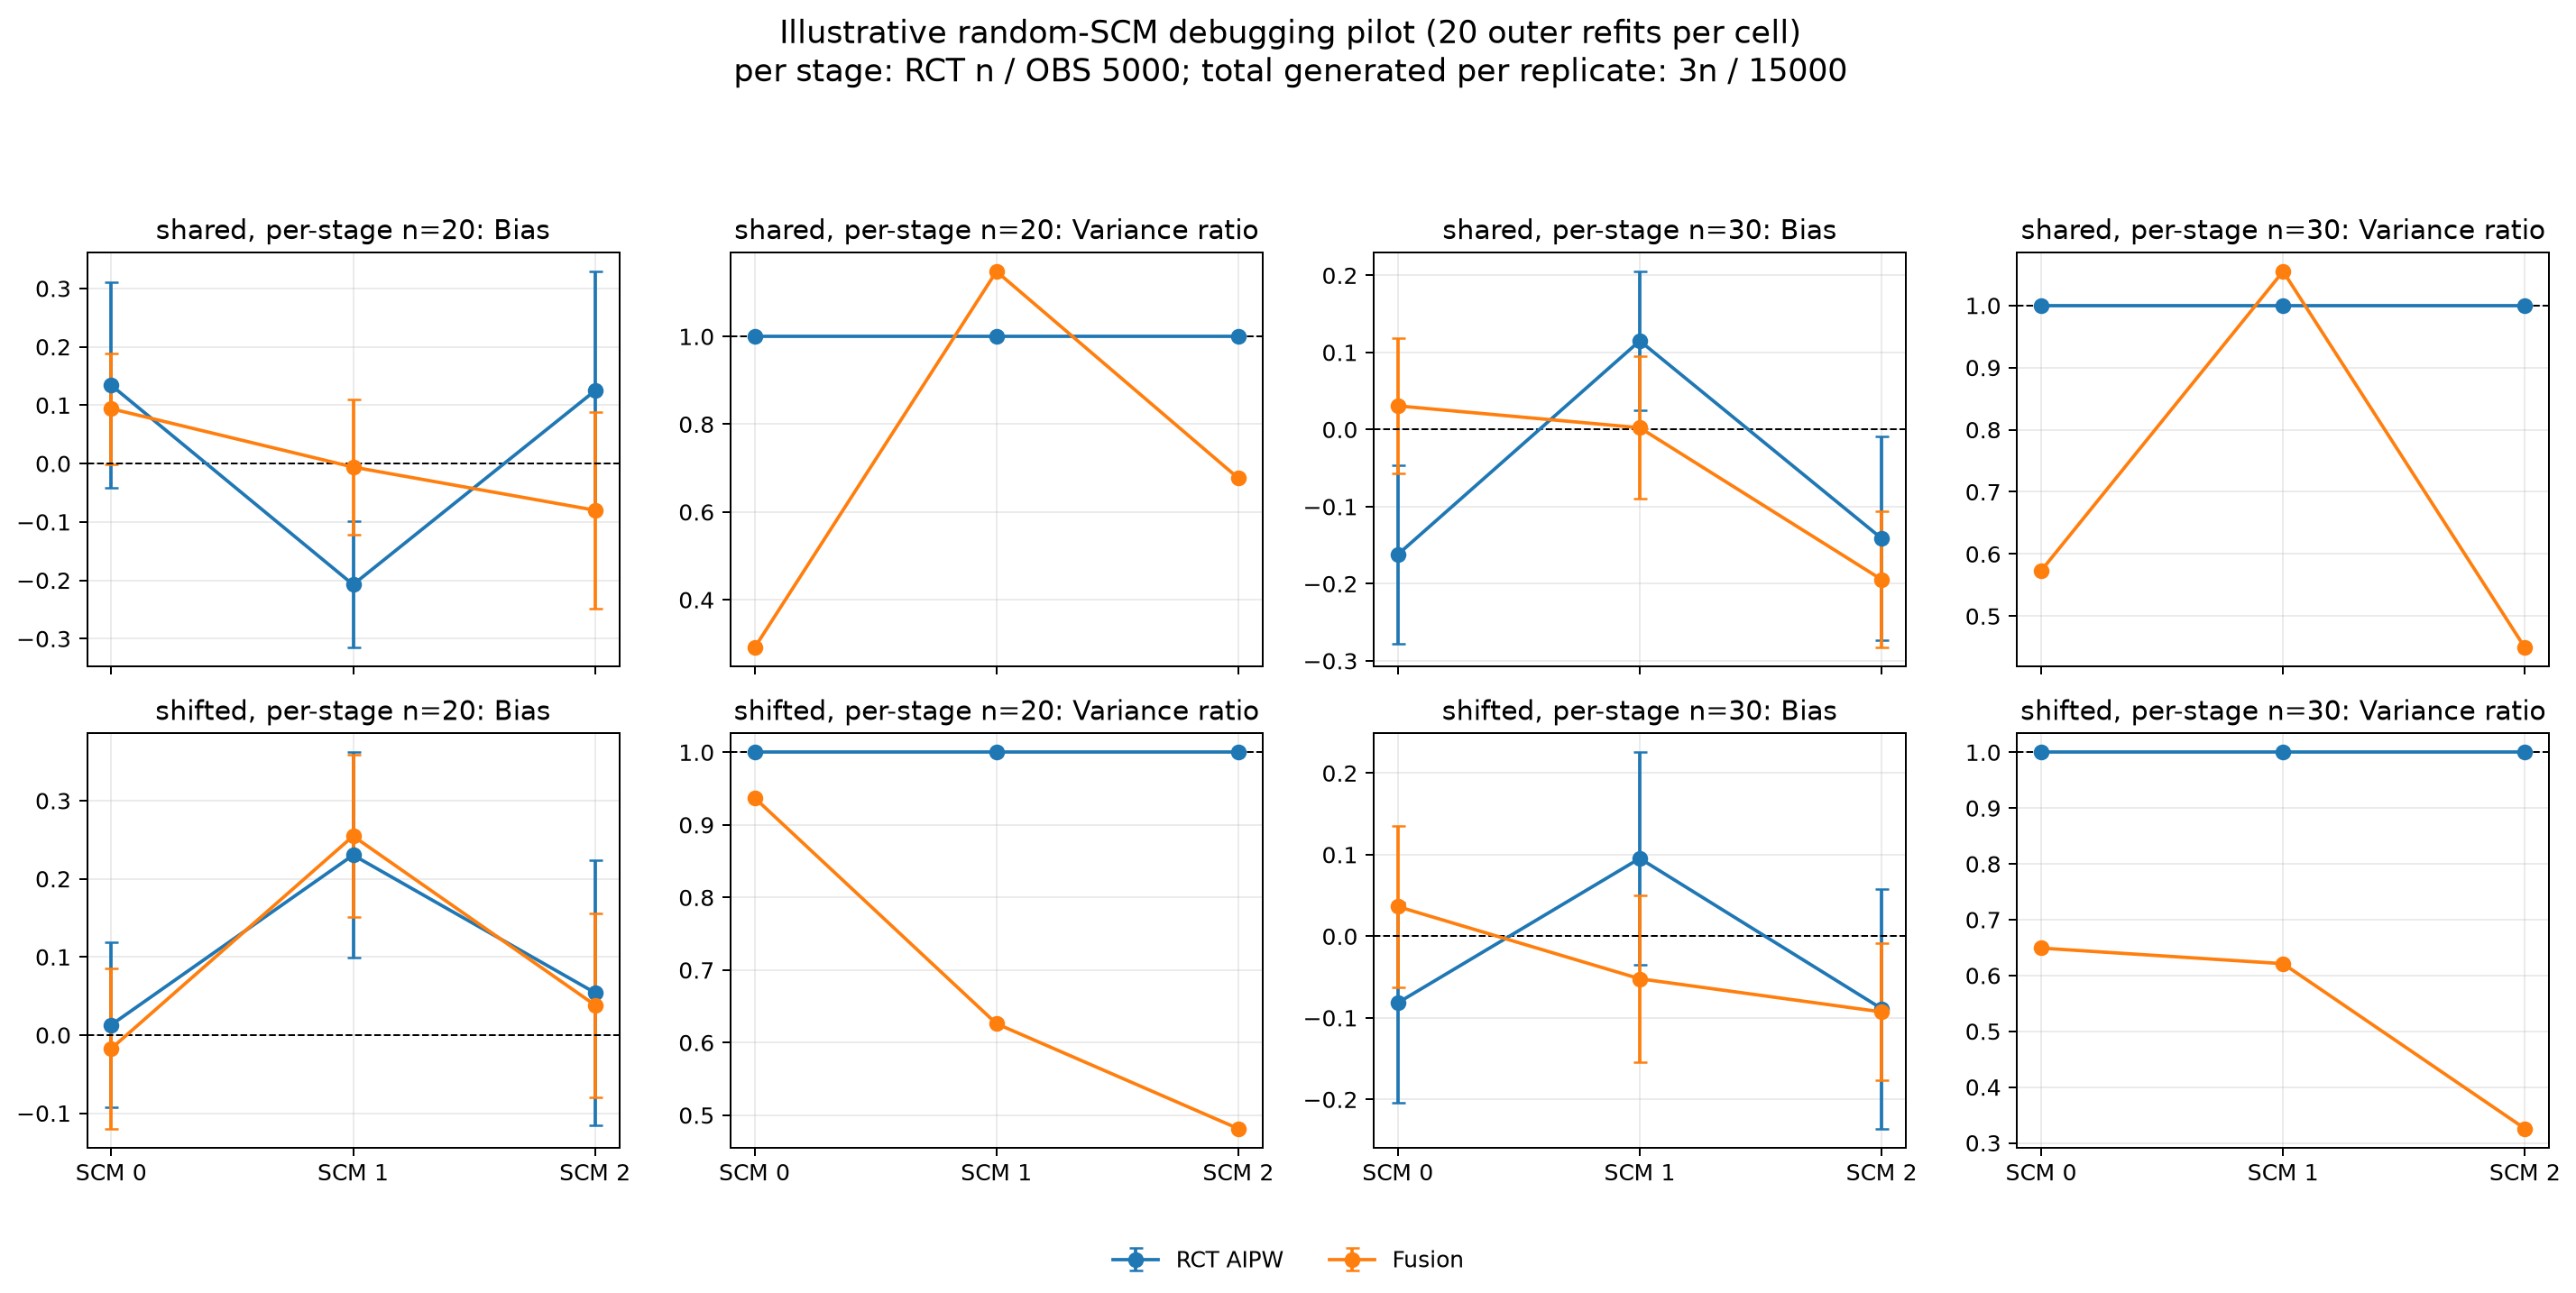
\includegraphics[width=0.98\textwidth]{../materials/ssem_ate_pilot.png}
\caption{Earlier SSEM ATE pilot.  This artifact predates the nested four-method
comparison and should be interpreted only as a design and implementation check.}
\label{fig:pilot}
\end{figure}

No participant-level WHI CT+OS analysis is included.  Such an analysis requires
authorized data access, a verified trial--observational semantic crosswalk, a
prespecified estimand, and methods appropriate for censoring if the selected
outcome is time-to-event.  No completed CATE experiment or real-outcome result is
represented by the present artifacts.
